\section{Efectul Compton}

Atunci când un fascicul de raze X, provenit de la o sursă $S$, trece printr-un
bloc de grafit $G$, radiațiile incidente sunt împrăștiate în toate direcțiile.

\begin{wrapfigure}[9]{r}{0.5\textwidth}
    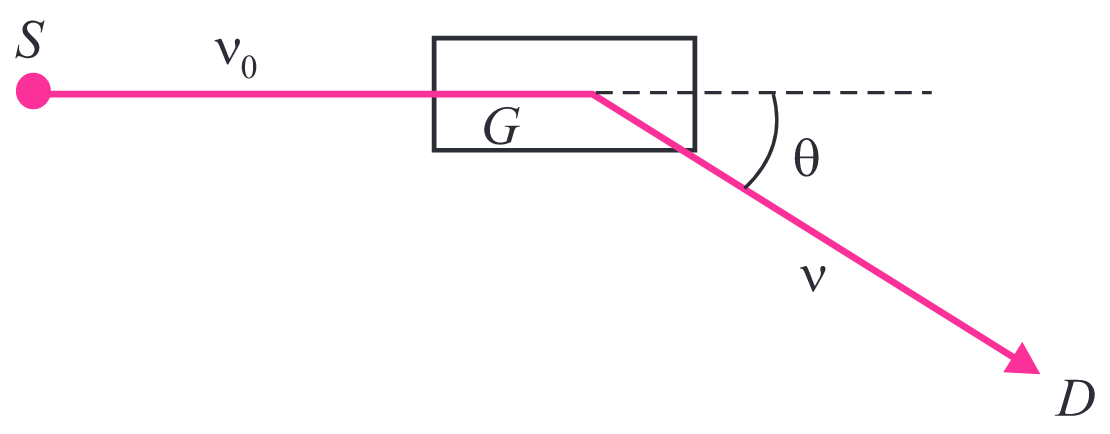
\includegraphics[width=0.5\textwidth]{fig/compton}
    \caption{Experimentul Compton, reprezentat schematic}
\end{wrapfigure}

Pentru diferite unghiuri de împrăștiere $\theta$, detectorul $D$ înregistrează,
pe lângă radiația incidentă cu lungimea de undă $\lambda_0$, și o altă radiație
cu lungimea de undă \( \lambda > \lambda_0 \).

Din punct de vedere macroscopic, lumina, și în general radiația electromagnetică,
este o undă. Din punct de vedere microscopic, lumina este un ansamblu de particule
cuantice.

\parbreak

Fenomenul, observabil pentru lungimi de undă mici, ca în cazul razelor X și
\gamma, deci pentru frecvențe mari (\(\lambda = \frac{c}{\nu} \)), a fost
explicat de către Compton pe baza naturii corpusculare a undelor electromagnetice,
adică prin existența fotonilor.

\emph{%
    Efectul Compton este fenomenul de împrăștiere elastică a fotonilor pe
    electronii liberi, în urma căreia, pe lângă radiația incidentă, apare și
    o radiație cu lungimea de undă mai mare (frecvența mai mică).
}

În cazul în care atomii substanței pe care se produce împrăștierea sunt ușori,
ca în cazul atomilor de siliciu, bor sau bariu, atunci energia de legătură a
electronilor de valență este mult mai mică decât energia fotonului incident
$h\nu_0$, iar electronul poate fi considerat practic liber.
